\section{リュカの定理とシェルピンスキーのギャスケット}

ここでは,\textsf{FD}から導かれるリュカの定理によって,パスカルの三角形を色分けしたものである「シェルピンスキーのギャスケット」を効率的に表示するアルゴリズムを作成する。また,Pythonを用いる。

\subsection{リュカの定理}
\begin{thm}[Lucas]
    非負整数$n,m$と素数$p$に対し,$0 \leqq n_i< p$の下で,\[
    n=n_kp^k+n_{k-1}p^{k-1}+\cdots+n_0p^0,\,m=m_kp^k+m_{k-1}p^{k-1}+\cdots+m_0p^0
    \]
    とする.このとき,\[
    \binom{n}{m}\equiv \prod_{i=0}^{k} \binom{n_i}{m_i} \quad \mathrm{mod}\, p
    \]
    である.ただし,$a<b$に対しては$\binom{a}{b}=0$とする.
\end{thm}

これがリュカの定理である。実はこれは,補題\ref{mod_fresh}を用いて示すことができる。具体的には,次の補題を用いる。
\begin{lemma}[\textsf{FD}]\label{mod_fresh_sec}
    $x\in\mathbb{Z}$に対し,$(1+x)^{p^i}\equiv 1+x^{p^i} \quad \mathrm{mod}\,p$である.
\end{lemma}

この補題は補題\ref{mod_fresh}を繰り返し用いれば容易に示せる。

それでは,この補題を使ってリュカの定理を証明していこう:
\begin{prf}
    $(1+x)^n$を展開した時の$x^m$の係数に注目することで示す.

    まず,$(1+x)^n=\prod_{i=0}^{k}(1+x)^{n_ip^i}\equiv\prod_{i=0}^{k}(1+x^{p^i})^{n_i}\quad \mathrm{mod}\,p$となる.また,$m=m_kp^k+m_{k-1}p^{k-1}+\cdots+m_0p^0$という表示の一意性より,最右辺で$x^m$という項が登場するのは,$(1+x^{p^k})^{n_k}$から$x^{m_kp^k}$,$(1+x^{p^{k-1}})^{n_{k-1}}$から$x^{m_{k-1}p^{k-1}}$,\dots,$(1+x^{p^0})^{n_0}$から$x^{n_0}$,を選出したもののみなので,$x^m$の係数は,$\prod_{i=0}^{k}\binom{n_i}{m_i}$である.よって,法$p$の下,$\binom{n}{m}\equiv\prod_{i=0}^{k}\binom{n_i}{m_i}$である.
\end{prf}

少々技巧的な証明だが,\textsf{FD}の威力が存分に発揮されているのが見て取れる。

ここで少し定理の条件に触れておく。$n=n_kp^k+n_{k-1}p^{k-1}+\cdots+n_0p^0,\,m=m_kp^k+m_{k-1}p^{k-1}+\cdots+m_0p^0$という表示は$p$進法を想起させる。コンピュータは2進法で動いてるよ,とかの話で出てくるアレだ。実際にその通りで,条件は$p$を基数としたときに$n=n_kn_{k-1}\cdots n_0,m=m_km_{k-1}\cdots m_0$であることと同じである。

\subsection{シェルピンスキーのギャスケット}
まず,シェルピンスキーのギャスケットについて説明する。

一言で言うと,パスカルの三角形を色分けしたものだ。一般的には偶奇で色分けしたものを言う。しかし,そもそもシェルピンスキーのギャスケットは,どれだけ拡大しても同じ構造が現れてくる「フラクタル図形」の一種である点が重要である。一度ネットなどで画像を調べたり,自分でパスカルの三角形を塗り分けてみたりして,その容貌を目に焼き付けてからこれ以降の内容を読んで欲しい(図\ref{sierp_2_and}を見てもらっても構わない)。

\vspace{10pt}

シェルピンスキーのギャスケットを表示する際に問題となるのは,二項係数の偶奇を判定する方法である。素朴にやるのであれば,\texttt{\textbf{import} math}のもとで\texttt{math.comb(n,m) \% 2}をひたすら計算すれば良いが,これでは,ギャスケットの段数が大きくなった時に時間がかかってしまう。そこで,リュカの定理をうまく使う。そのまま使うと,一度2進法に直したものを2で割ったあまりを求めて掛け合わせなければならないが,プログラム\ref{sierpinski}に示したアルゴリズムはより速いものである。なお,プログラムはこのpdfを載せたGitHubリポジトリ(\url{https://github.com/stochastic-yukke/sukenbushi2025})の「py\_files」の中に「using\_and.py」という名前で置いておきました。

\begin{lstlisting}[caption=uszczelka Sierpińskiego,label=sierpinski]
import matplotlib.pyplot as plt
import numpy as np

def binomial_odd(n: int, k: int):
    return (n & k) == k

def lucas_mod2_triangle(rows):
    triangle = np.zeros((rows, 2 * rows - 1), dtype=int)
    for n in range(rows):
        for k in range(n + 1):
            col = rows - n + 2 * k - 1
            triangle[n, col] = binomial_odd(n, k)
    return triangle

def plot_sierpinski_lucas(rows):
    data = lucas_mod2_triangle(rows)
    fig, ax = plt.subplots(figsize=(8, 8))
    ax.imshow(data, cmap='binary', interpolation='nearest')
    ax.axis('off')
    return fig

# 図を生成して表示
fig = plot_sierpinski_lucas(256)
plt.show()
\end{lstlisting}

結果は図\ref{sierp_2_and}のようになる。
\begin{figure}[ht]
    \centering
        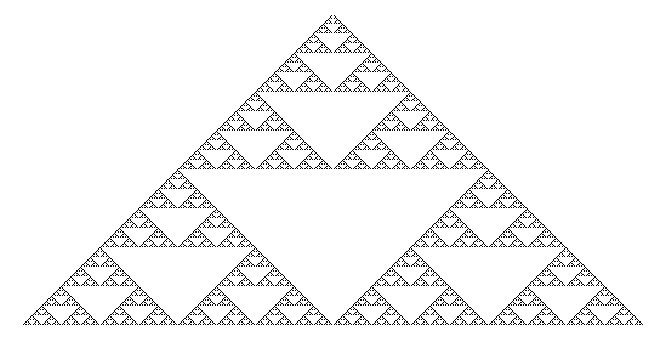
\includegraphics[scale=0.5]{Figure_using_and.png}
    \caption{シェルピンスキのギャスケット(mod2, rows=256)}
    \label{sierp_2_and}
\end{figure}

このプログラムにおいて注目して欲しいのは,4-5行目の関数\texttt{binomial\_odd}である。\texttt{\&}というのは,「論理積」を意味する。自然数$n$と$k$を二進法表記したときの$i+1$桁目の数の組$(n_i,k_i)$が$(1,1)$のときのみ1を,そうでないとき0を,その$i$桁目とするような数を,再び10進法にしたものが$n,k$の論理積である。例えば,$7=0111{}_{(2)},\,11=1011{}_{(2)}$だから,各桁を比較することで\texttt{7\&11}は$0011{}_{(2)}=3$であるとわかる。

$n,m$を$k+1$桁に二進展開したときの$i+1$桁目$n_i,m_i$に対する$\binom{n_i}{m_i}$としてありうるのは$\binom{1}{1}=1,\binom{1}{0}=1,\binom{0}{1}=0,\binom{0}{0}=1$のみであるから,リュカの定理より,$(n_l,m_l)=(0,1)$となるような整数$0\leqq l \leqq k$が存在する時,かつそのときに限り,$\binom{n}{m}\equiv 0 \quad \mathrm{mod}\,2$となる。したがって,$(n_l,m_l)=(0,1)$となる$l$の有無によって二項係数の偶奇を判定すればよい。実はここで,$\mathtt{\&}$が活躍する。$(n_l,m_l)$に対し,$n_l,m_l$の論理積を計算することを考えると,$n_l\mathtt{\&}m_l\ne m_l$となるのは,$(n_l,m_l)=(0,1)$のとき,かつその時に限るから,$n\mathtt{\&}m$の桁で,$m$の対応する桁と一致しないものが1つでもあれば,$\binom{n}{m}\equiv 0\quad \mathrm{mod}\,2$となり,$n\mathtt{\&}m$が$m$と一致するならば,$\binom{n}{m}\equiv 1\quad\mathrm{mod}\,2$となる。そういうわけで,このプログラムでは論理積によって二項係数の偶奇を判定しているのである。

\subsection{素数判定アルゴリズム「AKS判定法」の紹介}
\textsf{FD}が効果的に用いられている素数判定法がある。\textbf{AKS判定法}だ。今回は紹介するに留めるが,素数判定の歴史から鑑みても非常に重要なアルゴリズムである(\textbf{史上初の多項式時間で判定可能な決定的素数判定アルゴリズム})。

最も初等的な素数判定のやり方は,フェルマーの小定理を用いる「フェルマーテスト」だが,これでは完全に素数のみを抽出するアルゴリズムとは言えない(フェルマーの小定理の条件を考えればわかる)。このような,素数と合成数をきっぱり峻別できないようなアルゴリズムとは異なり,AKS判定法は確定的に素数を判定できる優れものだ。それでは,アルゴリズムの詳細を以下に示そう:

整数$n>1$に対して,
\begin{enumerate}
    \item $a\in \mathbb{N}が存在してn=a^bかつb>1$ならば「$n$は合成数」と出力して終了.
    \item $\mathrm{ord}_r(n)>\log^2n$をみたす最小の$r$を見つける.
    \item ある$a\leqq r$に対して,$1<(a,n)<n$であるならば「$n$は合成数」と出力して終了.
    \item $n\leqq r$ならば「$n$は素数」と出力して終了.
    \item $a$を$1$から$\lfloor\sqrt{\varphi(r)}\log n\rfloor$まで動かす.$(X+a)^n\not\equiv X^n+a \pmod {X^r-1,n}$ならば「$n$は合成数」と出力して終了.
    \item 「$n$は素数」と出力して終了.
\end{enumerate}

ただし,$(\cdot ,\cdot)$は二数の最大公約数,$\lfloor\cdot\rfloor$は床関数(その数を超えない最大の整数を示す記号),$\varphi$はオイラー関数(正整数$n$に対し,$n$と互いに素な1以上$n$以下の正整数の個数を与える関数)である。また,正整数$x$に対して,$\mathrm{ord}_r(x)$は,法$r$における$x$の位数である(定義\ref{def_genshikon}参照のこと)。

アルゴリズムの5. において\textsf{FD}が輝いているのが見えるだろうか。あれが星というものである。



